% Бүлэг 1

\chapter{Оршил} % Бүлгийн нэр
\label{Chapter1} % Энэ бүлэг рүү ишлэл хийх бол \ref{Chapter1} командыг ашигла 

% Агуулгад ашигласан хэвшүүлэлтийн зарим командын тодорхойлолт
\newcommand{\keyword}[1]{\textbf{#1}}
\newcommand{\tabhead}[1]{\textbf{#1}}
\newcommand{\code}[1]{\texttt{#1}}
\newcommand{\file}[1]{\texttt{\bfseries#1}}
\newcommand{\option}[1]{\texttt{\itshape#1}}

%-------------------------------------------------------------------------------
\section{Зорилго}
Их дээд сургуулиудын багш нар хичээлийн материал болон лабораторын удирдамжаа онлайн байршуулах зорилготой. 

	\section{Зорилтууд}
		\begin{itemize}
			\item Хэрэглэгчийн шаардлага тодорхойлно. 
			\item Интерфэйс html хуудас.
			\item Активити диаграм, модель классын код.
			\item ERD диаграм, контролёр классын код.
			\item Класс диаграм, харуулах хуудасны код php.
			\item Дарааллын диаграм, JS кодчилол.
			\item Бичиг баримт-сорил1.
			\item Тайлан, статистик код.
			\item Модулын нэгтгэл.
			\item Зүгшрүүлэлт
			\item Програм-сорил2
		\end{itemize}
	
	\section{Үнэлгээ}
		\begin{itemize}
			\item Найдвартай
			\item Уян хатан
			\item Ашигтай (Мэтгэлцээний клуб болон гишүүд мэдээллээ цахимаар авна)
			\item Хэрэглээтэй (Компьютерийн архитектураас үл хамааран ямар ч үйлдлийн систем дээр ажиллах боломжтой)
			\item Сайжруулалттай (цаашид засвар, шинэчлэлт хийх боломжтой)
			\item Үнэлгээ 	
		\end{itemize}


%------

%-------------------------------------------------------------------------------
\section{Хөгжүүлэлтэд ашиглах алгоритм}

\LaTeX{} бол Microsoft Word, Adobe Pages шиг \textsc{WYSIWYG} (Таны Харж байгаа Зүйл бол Таны Оруулсан Зүйл) төрлийн текст боловсруулах програм биш. \LaTeX{} --д зориулсан баримт нь үнэндээ \emph{хэвшүүлээгүй} задгай текст бүхий файл юм. Өөрийн тексттэй хамт түүнийг хэрхэн хэвшүүлэхийг тухай энгийн командыг бичиж, энэ файлаар \LaTeX{} --т хэлж өгдөг. Жишээ нь \emph{текстийг налуу болгож тодотгохдоо} \verb|\emph{text}| командыг ашиглах ба налуу болгох текстээ их хаалтанд бичнэ. Өөрөөр хэлбэл \LaTeX{} нь HTML -тэй маш төстэй ''{mark-up}'' хэл юм.

%-------------------------------------------------------------------------------

\section{Технологийн судалгаа}

	\subsection{MySQL}
	
	MySQL нь холбоост өгөгдлийн санг удирдах систем юм. MySQL хэмээх нэрний хувьд уг системийг санаачлан хөгжүүлэгч Micheal Widenius-ын охины нэр My + SQL(Structed Query Language) гэсэн утгатай ажээ.
	Энэ систем нь GNU (General Public License) буюу нээлтэй эхийн систем учир хүссэн хэн бүхэн хөгжүүлэлтэнд оролцож, үнэгүй хэрэглэж болох юм. Эзэмшигч нь алдарт Java-г хөгжүүлсэн Sun MicroSystems компани байсан ба, одоогоор Sun-г Oracle корпораци эзэмших болсон билээ.
	Үнэгүй програм хангамжийн өгөгдлийн санг удирдах системд ихэвчлэн MySQL-ийг хэрэглэдэг бөгөөд тэдгээрийн сонгодог жишээ гэвэл Joomla, Drupal, Wordpress, phpBB гэх мэт агуулга удирдах системүүд (CMS-Content Management System), Wikipedia, Facebook, Google гэх мэт томоохон компаниуд хэрэглэдэг юм.
	Хөгжүүлэлт нь C/C++ хэл дээр хийгдсэн ба AIX, BSDi, FreeBSD, HP-UX, i5/OS, Linux, Mac OS X, NetBSD, Novell NetWare, OpenBSD, OpenSolaris, eComStation, OS/2 Warp, QNX, IRIX, Solaris, Symbian, SunOS, SCO OpenServer, SCO UnixWare, Sanos, Tru64, Microsoft Windows гэсэн олон үйлдлийн системүүд дээр ажилладаг.
	MySQL бол хамгийн өргөн хэрэглээтэй нээлттэй эхийн (Open Source) өгөгдлийн сан удирдах програм юм. Анх 1995 онд зах зээлд гарсан ба с/с++ хэл дээр бичигдсэн. Одоогийн байдлаар 5.7 нь хамгийн сүүлийн хувилбар болон гараад байна. Энэ сүүлийн хувилбар дээр нэмэгдсэн давуу талууд гэвэл 3 дахин хурдан үйл ажиллагаатай болсон мөн натив JSON дэмжигчтэй болсон гэх мэт шинэлэг үйлдлүүд нэмэгдсэн байна.
	
	\subsection{Php}
	  Rasmus Lerdorf WWW-д вэб хуудас үүсгэх үедээ өгөгдөл боловсруулах хялбархан арга хайж байгаад 1995 онд PHP хэлийг скрипт хэл байдлаар зохиосон.
	PHP нь сервер талын скрипт хэл ба динамик вэб хуудас хийхэд илүү тохиромжтой. Энэ скрипт хэл нь энгийн хэрэглээний вэб сайтаас эхлээд байгууллагын иж бүрэн вэб программ хийж болохоор MySQL мэтийн өгөгдлийн сантай харилцан ажиллах боломжтой.
	Хуудас ачаалах үед броузерээр нэг бүрчлэн уншдаг HTML-тэй адилгүй, PHP баримтыг бэлтгэхдээ серверээр урьдчилан боловсруулдаг. PHP код агуулсан хуудас нь хэрэглэгчийн броузерт илгээгдхээс өмнө серверээр боловсруулагдсан байдаг.
	PHP хэлний өөр нэг давуу тал бол скриптэн хэл юм. Ихэнх програмчлалын хэлнүүдэд ажиллахын өмнө машины хэл рүү хөрвүүлэх тусгай файлууд /compile/ шаардлагатай байдаг бол PHP хэлний хувьд хөрвүүлэлт хийх шаардлагагүй байдаг тул код засварлах болон шалгахад илүү хурдан байдаг
	
	\subsection{Системийн судалгаа}
	Үндэслэл
		Мэдээллийн технологийнн ололт амжилттай уялдаж дэлхийн улс орнуудад цахим сургалт нь өргөн хүрээнд хэрэгжиж байна.
		Орчин үеийн технологид суурилсан сургалтын шинэ арга хэлбэрийг ашигллан цаг хугацаа, орон зайнаас үл хамааран боловсрол олгох, насан туршийн суралцах боломжийг бий болгох зорилгыг хэрэгжүүлэхэд шийдвэл зохих тулгамдсан асуудал бол нэгдсэнн стандарт бүхий э-хичээл боловсруулах шаардлагтай байгаа юм.
		
		Э-хичээл боловсруулах стандарт байхгүй тохиолдолд багш бүр өөр өөрийн хувилбараар боловсруулах ба энэ нь цахим сургалтын үр дүнд муугаар нөлөөлнө.
		
	Стандарт гэж юу вэ? 
		Стандарт нь хэмжээ, загвар гэсэн утгатай ба өргөн утгаараа үлгэрчилсэн загвар, эх хэмжүүр, бүдүүвчилсэн зураг гэсэн утгатай үг юм. Үүнийг онлайн сургалтанд дараах байдлаар тодорхойлдог байна. 
		
		Э-хичээлийн стандарт-----------------------нийтлэг дагаж мөрдөх дүрэм журмын багц юм. 
		
	Онлайн хичээл явуулахад анхаарах техникийн шаардлагууд
	
		Сургалтанд ашиглагдах онлайн сургалтын систем нь бүх хэрэглэгчидэд хүртээмжтэй, энгийн щ, ашиглахад хялбар байх. 
		Интернэтийн хурдаас үл хамааран суралцагч гэрээсээ, сургуулиасаа аль ч үед хандаж суралцах боломжтой. 
		Нийтлэг ашиглагддаг үйлдлийн систем болох Windows болон Mac үйлдлийн системүүдийн аль алинд нь зохицож ажиллаж болдог байх.
		Видео болон аудио файлын хэмжээ нь 8MB-аас ихгүй байх.
		Текстэн материалууд нь суралцагчдад хүртээмжтэй стандарт форматаар хангагдсан байх.
		Суралцагч өөрийн компьютераасаа хичээлийн материалыг хэвлэж, хадгалж болохуйцаар агуулгад шигтэж өгсөн байх.
		Болж өгвөл үнэгүй эсвэл лицензтэй программ хангамж ашигласан байх.
		
	Дэлгэцийн зохиомждоо дараахыг анхаарах
	
		Хичээлийн текстийг дэлгэцэнд бүтнээр нт багтаа. Энэ нь уншиж боловсруулахад төхөм болно.
		Текстийн хэмжээг 5-8 мөрөөр хязгаарлаж, 15-аас дээш мөр оруулахгүй байж, 8 хүртэлх үгийг нэг мөрөнд багтаах.
		Дэлгэцэнд текстийн 1 ба 2-оос илүү хэлбэртэй параграф оруулахгүй байх.
		Хэрэглэхэд ойлгомжтой, энгийн байх(ээдрээтэй, эргэлзээтэй би).
		Өртөг зардал, цаг хугацаа хэмнэсэн байх.
		
	Дүгнэлт 
	
		Лекцийн бүтэц, технологи нь цаг үеийн шаардлагыг даган өөрчлөгдөж боловсронгуй болж байх ёстой зүйлийн нэг мөн.
		Судлаачдын тогтоосоноор лекцийн явцад оюутнуудын анхаарал 10-15 минутын давтамжтай 2-3 удаа буурдаг байна.
		Лекцийн хичээлийн чанарыг сайжруулахын тулд суралцагчдын сурах сэдлийг бий болгох явдал чухал үүрэгтэй.
		Семинар болон лабораиорын хичээл нь оюутны мэдлэгийг бататгах, гүнзгийрүүлэх, өргөжүүлэх, мэдлэгээ амьдралдаа хэрэглэх арга барил, чадвар дадал олгох үүрэг зориулалттай сургалтын зохион байгуулалтын нэг хэлбэр юм.
		\newpage
		\subsubsection{Оюутны вэб}
		\begin{figure}
			\centering
			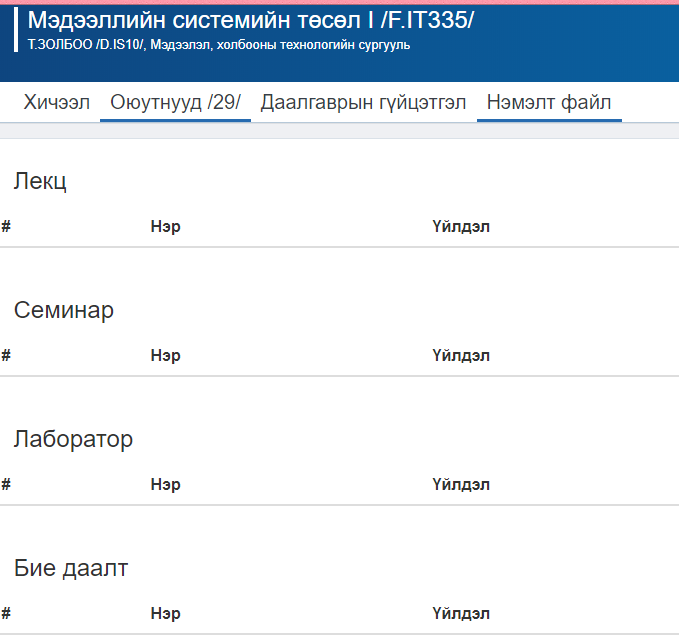
\includegraphics[scale=0.5]{Diagrams/Sudalgaa1}
			\caption[Оюутны вэб https://student.cloudmis.edu.mn/Login]{Оюутны вэб https://student.cloudmis.edu.mn/Login}
			\label{text}
		\end{figure}
	
		\newpage
		\subsubsection{ШУТИС МХТС Цахим сургалт}
		\begin{figure}
			\centering
			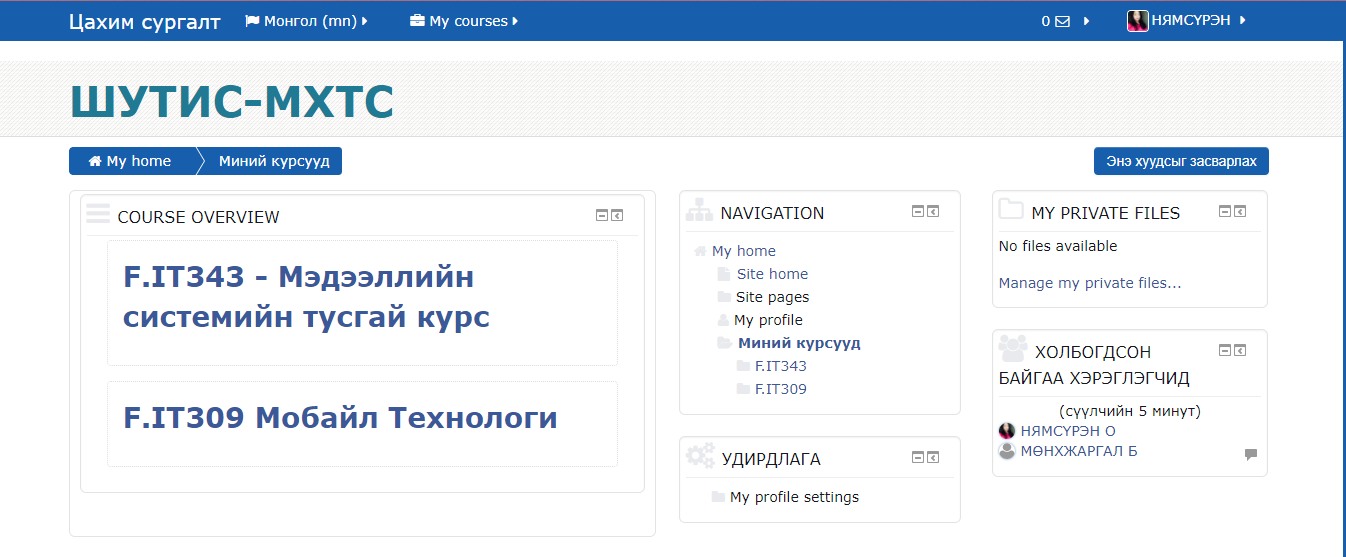
\includegraphics[scale=0.5]{Diagrams/Sudalgaa2}
			\caption[Цахим сургалт http://elearn.sict.edu.mn/login/index.php]{Цахим сургалт http://elearn.sict.edu.mn/login/index.php}
			\label{text}
		\end{figure}
		
			\newpage
		\subsubsection{ШУТИС МХТС Цахим сургалт}
		\begin{figure}
			\centering
			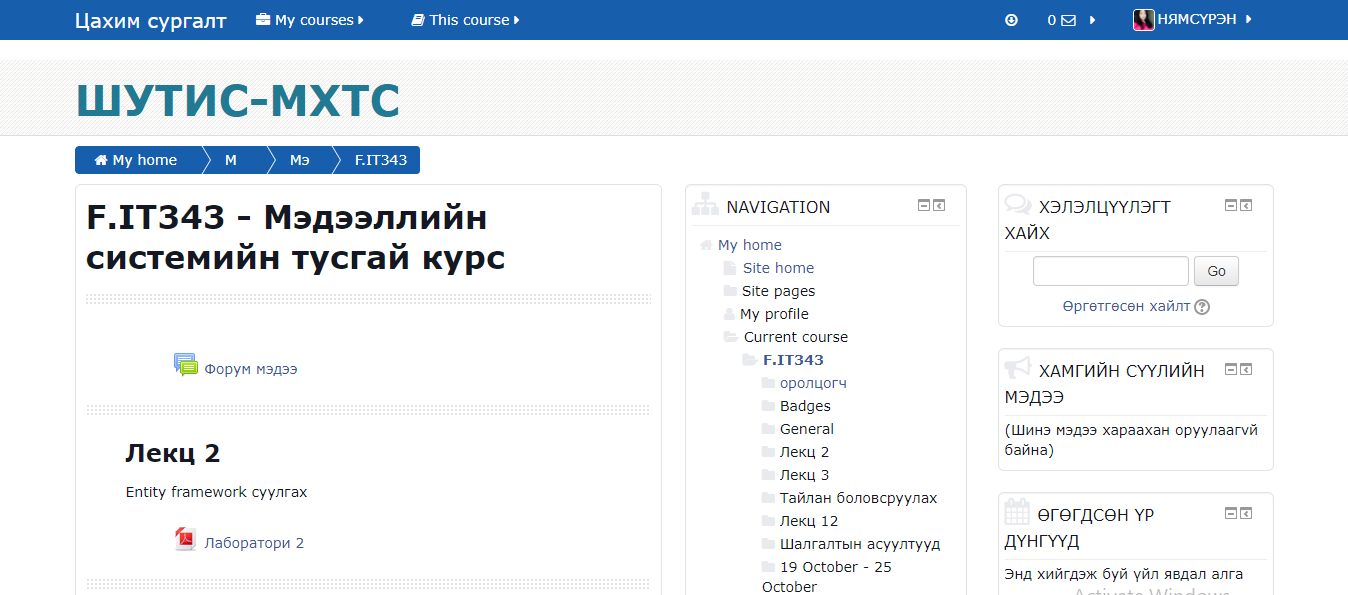
\includegraphics[scale=0.5]{Diagrams/Sudalgaa3}
			\caption[Цахим сургалт http://elearn.sict.edu.mn/login/index.php]{Цахим сургалт http://elearn.sict.edu.mn/login/index.php}
			\label{text}
		\end{figure}
\section{Бүлгийн дүгнэлт}

	Энэ бүлэгт өөрийн хийх гэж буй вэбийн зорилго зорилт болон ашиглах програмчлалын хэл болон архитектурын судалгаа, онол агуулгын мэдээллээ орууллаа.
%-------------------------------------------------------------------------------